\subsection{Matching based solutions} 

In the simplest version of $\Problem$, where all properties are absent, each VM 
is allready placed, the loactions of all chunks are known, and we have to 
compute an assignment of VMs to chunks, such that each VM is assigned to 
exactly one chunk, and each chunk is assigned to exactly one chunk. Hence we 
can transform each instance of $\Problem$ to a minimum weight perfect bipartite 
matching problem. One of the sets is formed by $\VirtualNodes$, the other by the 
set of chunks. A VM has an edge to each chunk. The costs of these edges are 
defined by the hop count between the VM and the chunk in the host graph. Each 
edge which is chosen for the solution of the matching problem, indicates that 
the chunk is assigned to the vm of the edge.

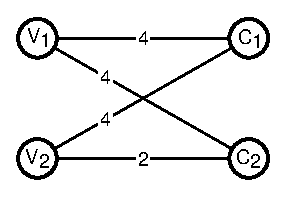
\includegraphics[angle=90,origin=c, 
height=7cm]{figs/model_fig_skteches/matching_basic}

This approach can also be used to solve instance of $\Problem$, which have the 
$ma$ or $r$ property - or even both. 
To Account for the $ma$ property, a single VM has to process exactly 
$\MaFactor$ VMs. Hence we can clone a VM to be represented by $\MaFactor$ Nodes.
In order to incorporate the different 
replicas of the chunks, we depict all copies of a given $\ChunkTypes$ in a 
single %$\ChunkType$ 
node. We connect each VM to all $\ChunkTypes$ using the 
lowest hop count to one of the copies as the weight.

Many algorithms solve the minimum weith perfect matching problem on bipartite 
graphs. The algorithms runtimes depend on  the number of nodes in the 
graph $n$, the number of edges in the graph $m$, and the largest magnitude of 
an edge weight $N$. An efficient algorithm is described by Gabow et al. in 
\cite{gabow_scaling_algorithm} and provides a runtime of $\mathcal{O}(n^{3/4} 
\cdot m \cdot \log n)$ which translates to $\mathcal{O}((\MaFactor \cdot \Vms + 
\ChunkTypes)^{3/4} \cdot  \MaFactor \cdot \Vms \cdot \ChunkTypes \cdot \log 
(2 \cdot h(\Tree)))$, where $h(T)$ denotes the height of the tree.